\documentclass[12pt]{article}
\usepackage[print,nopanel]{pdfscreen}
\begin{print}
\usepackage{lastpage}
\usepackage{macro/macro}

\usepackage{fancyhdr}
\usepackage{verbatim}
\lhead{\large\bfseries Souvenir}
\usepackage[left=2.5cm, right=1.5cm, top=1.5cm, bottom=1.5cm]{geometry}
\pagestyle{fancy}
\end{print}
\margins{.5cm}{.5cm}{.5cm}{.5cm}
\begin{screen}

\renewcommand{\encodingdefault}{T1}
\usepackage{setspace}
\linespread{1.5}
\renewcommand{\rmdefault}{ptm}
\end{screen}
\screensize{8cm}{9cm}
\overlay{overlay8.pdf}
\usepackage{graphicx}

\begin{document}
\newcommand{\centertext}[1]{\begin{center}\textbf{#1}\end{center}}
\newcommand{\student}{\vskip 2.5cm}
\newcommand{\supervisor}{\vskip 2cm}
\newcommand{\stamp}{\vskip 2.5cm}
\newcommand{\projecttitle}{\Huge \bf{Souvenir\\{Yaadein: Preserving Memories}}\vskip 0.5in}

\newcommand{\logo}[1]{\includegraphics[scale=0.7]{#1}}
\newcommand{\submitted}{
\vskip 0.4in
Submitted In Partial Fulfillment Of The Requirement For\\
Six Weeks Training\\
at\\
Testing and Consultancy Cell, GNDEC\\
(from June, 2013 to July, 2013)\\
Batch:2011-2015\\
\vskip 1.5cm
%\image{0.7}{images/gne.jpg}{}
\logo{images/gne.jpg}
\vskip 1.5cm
\begin{flushleft}
Submitted By: \hspace{8cm} Submiited To:\\ 
Deepak Kumar Sharma\\
D$3$ I.T\\
1144685\\
\end{flushleft}
\vskip 1.2cm
\bf{Department of Information Technology} \\
\bf{GURU NANAK DEV ENGINEERING COLLEGE} \\
LUDHIANA-141006
}

\newcommand{\pagetitle}{\begin{center}
\projecttitle
\Large\textbf{Project Report}\\
\submitted
\vskip 1cm

\end{center}}
\newcommand{\openoffice}{\textbf{OpenOffice}}
\newcommand{\frontmatter}[1]{\begin{Large} \textbf{#1} \end{Large}}
\newcommand{\ppttitle}{\begin{center}
\Huge Souvenir
\vskip 1cm
\large Deepak Kumar Sharma
\vskip 0.3cm
\large Guided by: Dr. H.S. Rai
\vskip 0.3cm
\large deeky.sharma@gmail.com
\end{center}}


\begin{screen}
\ppttitle
\end{screen}
\footskip 0.7cm
\thispagestyle{empty} 
\pagetitle
\newpage
\pagenumbering{Roman}
\cfoot{\thepage}

%\begin{Large}
\centertext{To whom it may concern }
\end{Large}
I here by certify that Deepak Kumar Sharma Roll No. 1144685 of Guru Nanak Dev Engineering
College Ludhiana, has undergone six weeks training from June, 2013 to July, 2013 at
our organisation to fulfill the requirements for the award of six weeks traning of B.Tech (D3 I.T.).
He worked on Souvenir (‘Yaadein: Preserving Memories’) project during the training under the
supervision of Dr. H.S. Rai (Dean, Testing and consultancy Cell, Guru Nanak Dev
Engineering College). During his tenure with us we found him sincere and hard working. We wish him great success in the future.
\vskip 2.0cm
Signature of the Student\\
\vskip 2.0cm
Signature of the Supervisor\\
\vskip 2.0cm
(Seal of Organisation)


\newpage
\begin{Huge}
\centertext{Acknowledgement}
\end{Huge}
I, student of Guru Nanak Dev Engineering College, Ludhiana, have taken efforts in this project. However, it would not have been possible without the kind support and help of many individuals and organizations. I would like to extend my sincere thanks to all of them.\\\\
The author is highly grateful to Dr. M.S. Saini Director, Guru Nanak Dev Engineering College, Ludhiana for providing him with the opportunity to carry out his Six Weeks Training at Testing and Consultancy Cell, Guru Nanak Dev Engineering College, Ludhiana.\\\\
The author would like to whole heartedly thank Dr. H.S. Rai Dean, Testing and Consultancy Cell, Guru Nanak Dev Engineering College, Ludhiana who is a vast sea of knowledge and without whose constant and never ending support and motivation, it would never have been possible to complete the project and other assignments so efficiently and effectively.\\\\


\newpage
\begin{Large}
\centertext{Abstract}
\end{Large}
‘Yaadein: Preserving Memories’ is a research and development project started with the
sole objective of automating the making of the Souvenir booklet which is given to all
passing out students. Research and Development refers to ‘creative work undertaken on
a systematic basis in order to increase the knowledge base regarding the knowledge of
man, culture and society, and the use of this knowledge to devise new and improved applications’. This project focuses on the automation and fast typesetting of the Souvenir
making process along with easy to use options for customizing the look and feel as well
as the layout of the souvenir. \\
\\
Yaadein is a great application to produce web based as well as printed copies of
souvenirs which are given to students when they pass out from schools and colleges.
It contains every students personal details, photograph, contact details and the comments/views of other students about them.\\ 
\\
Yaadein was made keeping in mind the various schools and colleges who spend several
man hours, which often run into days and sometimes weeks, designing their souvenir.
This project will not only help them significantly reduce the time consumed in the designing of the souvenir but will also make the overall process very simple and easy to
use. The Yaadein project is a highly customizable application that allows the user to
modify the look and feel of the souvenir as per their personal preferences.\\
\\
The motive of the project is to reduce the time consumed and to enable fast and
easy customization and even faster modifications when required as instead of typing and
scaling, only values in the php script need to be changed.\\
\\
Also, this project is completely open source and is made using PHP,\LaTeX{} version
\LaTeX{}2e and MySQL and the entire code is available to the user ,for fast and easy customization, as and when required. This project is governed by the GNU General Public
License v3.0 GNU-GPLv3.0.


\newpage
\tableofcontents
\newpage
\listoffigures
\newpage

\pagenumbering{arabic}
\cfoot{\thepage}

\newpage
\section{Introduction To Organisation}
\image{0.7}{images/gndec.jpg}{Guru Nanak Dev Engineering College}
\hspace{-1.7em} I am having my Six Months Industrial Training at TCC-Testing And Consultancy Cell, GNDEC Ludhiana. Guru Nanak Dev Engineering College was established by the Nankana
Sahib Education Trust Ludhiana. The Nankana Sahib Education Trust i.e NSET
was founded in memory of the most sacred temple of Sri Nankana Sahib, birth place
of Sri Guru Nanak Dev Ji. With the mission of Removal of Economic Backwardness
through Technology Shiromani Gurudwara Parbandhak Committee i.e SGPC started a
Poly technical was started in 1953 and Guru Nanak Dev Engineering College was established in 1956.\\\\
NSET resolved to uplift Rural areas by admitting 70% 
of students from these rural
areas ever year. This commitment was made to nation on 8th April, 1956, the day
foundation stone of the college building was laid by Dr. Rajendra Prasad Ji, the First
President of India. The College is now ISO 9001:2000 certified.\\\\
Guru Nanak Dev Engineering College campus is spread over 88 acres of prime land
about 5 Km s from Bus Stand and 8 Km s from Ludhiana Railway Station on Ludhiana-Malerkotla Road. The college campus is well planned with beautifully laid out tree plantation, pathways, flowerbeds besides the well maintained sprawling lawns all around. It
has beautiful building for College,Hostels,Swimming Pool,Sports and Gymnasium Hall
Complex, Gurudwara Sahib, Bank, Dispensary, Post Office etc. There are two hostels
for boys and one for girls with total accommodation of about 550 students. The main
goal of this institute is:\\\\
\begin{itemize}
\item To build and promote teams of experts in the upcoming specialisations.
\item To promote quality research and undertake research projects keeping in view their
relevance to needs and requirements of technology in local industry.
\item To achieve total financial independence.
\item To start online transfer of knowledge in appropriate technology by means of establishing multipurpose resource centres.
\end{itemize}
\subsection{Testing and Consutancy Cell}
My Six Months Institutional Training was done by me at TCC i.e Testing And
Consultancy Cell,
GNDEC Ludhiana under the guidance of Dr. H.S.Rai Dean Testing and Consultancy Cell.
Testing and Consultancy Cell was established in the year 1979 with a basic aim to produce
quality service for technical problems at reasonable and affordable rates as a service to society
in general and Engineering fraternity in particular.\\
\image{0.9}{images/aw.jpg}{Testing and Consultancy Cell}
\hspace{-1.3em} Consultancy Services are being rendered by various Departments of the College to the
industry, Sate Government Departments and Entrepreneurs and are extended in the form o5
expert advice in design, testing of materials \& equipment, technical surveys, technical audit,
calibration of instruments, preparation of technical feasibility reports etc.
This consultancy cell of the college has given a new dimension to the development
programmers of the College. Consultancy projects of over Rs. one crore are completed by the
Consultancy cell during financial year 2009-10. \\ \\
Ours is a pioneer institute providing Consultancy Services in the States of Punjab, Haryana,
Himachal, J\&K and Rajasthan. Various Major Clients of the Consultancy Cell are as under:\\
\begin{itemize}
\item Larson \& Turbo.
\item Multi National Companies like AFCON \& PAULINGS.
\item Power Grid Corporation of India.
\item National Building Construction Co.
\item Punjab State Electricity Board.
\item Punjab Mandi Board.
\item Punjab Police Housing Corporation.
\item National Fertilizers Ltd.
\end{itemize}


\newpage
\section{Introduction}
\begin{figure}[h!]
\centering

\includegraphics[width=0.9\textwidth]{images/cad1.png}
\caption{CAD}
\end{figure}
\hspace{-1.6em} Computer-aided design (CAD) is the use of computer programs to create two- or three-dimensional (2D or 3D) graphical representations of physical objects. CAD software may be specialized for specific applications. CAD is widely used for computer animation and special effects in movies, advertising, and other applications where the graphic design itself is the finished product. CAD is also used to design physical products in a wide range of industries, where the software performs calculations for determining an optimum shape and size for a variety of product and industrial design applications.\\\\
Hundreds of thousands of professionals in (take a deep breath) architecture, construction, engineering, commercial interiors, light construction, landscape architecture, kitchen and bath design, urban planning, game design, film and stage, woodworking, and plenty of other fields use CAD softwares all the time, every day.\\\\
GDCAD is a such application that can tackle with 2-D and 3-D graphics. GDCAD is like a pencil with superpowers. Start by drawing lines and shapes. Push and pull surfaces to turn them into 3D forms. Stretch, copy, rotate and paint to make anything you like. GDCAD is as simple and as powerful as you want it to be.\\\\
GDCAD uses set of toolbuttons and menu options to capture the CAD functionality. It has various toolbuttons to capture the implementation of various entities such as line, circle. point, ellipse etc. It has a drawing area with in which the entities are painted. The click of any toolbutton such as point button or other captures and stores the mouse positions, such that along that points things get painted. Also the mouse movements in the drawing area are captured and shown in the status bar. We can repaint the same entity again without having the need to click that button again. The signal from the same button remains active until and unless another button is clicked. Along with toolbuttons the menu also has the options to provide the painting of things. The shortcuts for each action are also implemented.\\\\
GDCAD also provides with the functionality of zooming in and out with the mouse scroll and same is also provided in the menu options.
It can also open, load and display an image with .jpg and .png format as sometimes the architectures and other need to have an idea by looking into the image. So no need to load it externally, GDCAD exhibits this feature. You can even select the entities or the area you want.\\\\
GDCAD is also designed to play nice with other software. So if you need to send your work to someone who needs a CAD file, you can use it to export pages as DWG and DXF files. It also exports multi-page PDFs also.\\\\
Every document you create has a physical paper size that you specify at the very beginning of your project. Because of this, all you need to do to print a plan view of your model at an exact scale is insert and set up a model viewport, and choose File then Print. It’s literally a two minute process.\\
% \begin{itemize}
% \item Format of the product: The size of the finished page determines how many pages
% can be printed on a single sheet.
% \item Number of pages of the printed product: The compositor must determine how
% many sheets are to be printed to create a finished book.
% \item Stitching/binding method: The compositor must understand how the sheets are
% placed to form the signatures that compose the finished book.
% \item Paper fiber direction: Many papers have a ”grain,” reflecting the alignment of the
% paper fibers. That these fibers must run lengthwise along the fold influences the
% alignment, hence the position, of the pages on the printed sheet.
% \item Finishing and binding
% \end{itemize}
% To understand how the pages are related to each other, an imposition dummy may be
% used. This is made by folding several sheets of paper in the way the press will print and
% fold the product. A little copy is then created, and this can help paginate the product.\\\\
%\image{0.9}{images/imposition.png}{Imposition of 16 pages}\\\\
\hspace{-1.8em} Also, this project is completely open source and is made using Qt as IDE, that uses the Qt libraries 
and the Qtwidgets with C++ and with openGl functionality, the entire code is available to the user as and when required.
The project is governed by the GNU General Public License v3.0 i.e GNU-GPLv3.0.\\\\
Various tools used to develop the project are:\\
\begin{itemize}
\item Qt version 4.7 or higher
\item C++
\end{itemize}

\section{Introduction to FEM}
In mathematics, the finite element method (FEM) is a numerical technique for finding approximate solutions to boundary value problems for differential equations. It uses variational methods (the calculus of variations) to minimize an error function and produce a stable solution. Analogous to the idea that connecting many tiny straight lines can approximate a larger circle, FEM encompasses all the methods for connecting many simple element equations over many small subdomains, named finite elements, to approximate a more complex equation over a larger domain.
\subsection{Finite Element Analysis}
Finite element analysis (FEA) is a computerized method for predicting how a product reacts to real-world forces, vibration, heat, fluid flow, and other physical effects. Finite element analysis shows whether a product will break, wear out, or work the way it was designed. It is called analysis, but in the product development process, it is used to predict what is going to happen when the product is used.\\
FEA works by breaking down a real object into a large number of finite elements, such as little cubes. Mathematical equations help predict the behavior of each element. A computer then adds up all the individual behaviors to predict the behavior of the actual object.\\
\subsection{FEM Software-Calculix}
CalculiX is a package designed to solve field problems. The method used is the finite element method.
With Calculix Finite Element Models can be build, calculated and post-processed. The pre- and post-processor is an interactive 3D-tool using the openGL API. The solver is able to do linear and non-linear calculations. Static, dynamic and thermal solutions are available. Both programs can be used independently. Because the solver makes use of the input format it is possible to use commercial pre-processors as well. In turn the pre-processor is able to write mesh related data for nastran, abaqus, ansys, code-aster and for the free-cfd codes duns, ISAAC and OpenFOAM. A CAD interface is available. The program is designed to run on Unix platforms like Linux and Irix computers but also on MS-Windows.\\
Calculix is a very powerful tool of analysis, highly configurable allowing the user to have complete control over the analysis, with more than 18 types of analysis covering most fields of study finite element Calculix's user can modify any variable on the analysis at discretion, the huge amount of information and documentation on the web make calculix a great alternative for the development of research projects where computer tools must accommodate the needs of the study.
\section{Introduction to DXF}
DXF stands for Drawing Exchange Format. Files that contain the .dxf file extension contain CAD vector image files.
The DXF file format is similar to the DWG file format, but DXF files are ASCII based and are therefore more compatible with other computer applications.The DXF file format was developed as an exchange format for the CAD files that are created by computer aided drafting software applications. The file format was initially introduced in December of 1982 as a part of AutoCAD 1.0. The file format was meant to provide an exact representation of the data in the standard AutoCAD file format.
\subsection {General File Structure}
A Drawing Interchange File is simply an ASCII text file with a file type of .dxf and specially formatted text. The overall organization of a DXF file is as follows:
\begin{itemize}
\item HEADER section--General information about the drawing is found in this section of the DXF file. Each parameter has a variable name and an associated value.

\item TABLES section--This section contains definitions of named items.

* Linetype table (LTYPE)

* Layer table (LAYER)

* Text Style table (STYLE)

* View table (VIEW)
* User Coordinate System table (UCS)

* Viewport configuration table (VPORT)

* Dimension Style table (DIMSTYLE)

* Application Identification table (APPID)

\item BLOCKS section--This section contains Block Definition entities describing the entities that make up each Block in the drawing.

\item ENTITIES section--This section contains the drawing entities, including any Block References.

\item END OF FILE
\end{itemize}



% \subsection{Limitations of Existing system}
% \begin{itemize}
% \item Operating System: Linux/Windows
% \item IDE: Qt version 4.7 or higher
% \item Programming Language:C++
% \end{itemize}


\newpage
\section{Django}
\subsection{Introduction to Django}
\image{0.2}{images/dl.png}{Django Logo}
\hspace{-1.8em} Django is an open source web application framework written in python. It lets 
you build high-performing, elegant Web applications quickly. Django 
focuses on automating as much as possible. Django's primary goal is to 
ease the creation of complex, database-driven websites. Django 
emphasizes reusability and "pluggability" of components, rapid 
development, and the DRY principal. Python is used throughout, even 
for settings, files, and data models. Django also provides an optional
 administrative create, read, update and delete interface that is 
generated dynamically through introspection and configured via admin 
models.\\\\
Django takes it name from the early jazz guitarist Django Reinhardt, 
a gypsy savant who managed to play dazzling and electrifying runs on 
his instrument even though two of the fingers on his left hand were 
paralyzed in an accident when he was young.\\\\
Thus, it’s a fitting name for the framework: Django can do some very 
complex things with less code and a simpler execution than you’d expect. 
It doesn’t take a heavy hand to build with Django. The framework does 
the repetitive work for you, allowing you to get a working website up 
quickly and easily.
\subsubsection{Installation of Django}
Installation of Django is also very easy.
The Django version is: Django 1.4.\\
Type the commands in the terminal:\\

	\$ wget http://www.djangoproject.com/download/1.4.5/tarball\\


	\$ tar xzvf Django-1.4.5.tar.gz\\


	\$ cd Django-1.4.5\\


	\$ sudo python setup.py install \\

\noindent This will install the django on your pc/laptop.

\noindent \subsubsection{MTV} Django adopts the standard 
MVC called Model-View-Controller design pattern. But instead, their naming 
convention is the MTV called Model-Template-View.\\\\
\begin{itemize}
\item \underline {Model} is an object relational mapping to your 
database schema. So each model is a class which represent a table in 
your database. Django models provide easy access to an underlying data 
storage mechanism, and can also encapsulate any core business logic, 
which must always remain in effect, regardless of which application is 
using it. Models exist independent of the rest of the system, and are 
designed to be used by any application that has access to them. In 
fact, the database manipulation methods that are available on model 
instances can be utilized even from the interactive interpreter, 
without loading a Web server or any application-specific logic.

\item \underline {Template} is simply HTML for your views. It also 
allows you to display different messages depending on whether or not a 
user logged in. Templates are Django’s provided way of generating 
text-based output, such as HTML or emails, where the people editing 
those documents may not have any experience with Python. Therefore, 
templates are designed to avoid using Python directly, instead favoring 
an extensible, easy-to-use custom language built just for Django.

\item \underline {View} could be a homepage or a page to display a 
user's information, for instance. A view accepts user input, including 
simple requests for information; behaves according to the application’s 
interaction logic; and returns a display that is suitable for users to 
access the data represented by models.
\end{itemize}

\subsubsection{Creating Project in Django}
If this is your first time using Django, you’ll have to take care of 
someinitial setup. Namely, you’ll need to auto-generate some code that 
establishes a Django project – a collection of settings for an instance 
of Django, including database configuration, Django-specific options 
and application-specific settings. From the command line, cd into a 
directory where you’d like to store your code, then run the command \\\\
\$ django-admin.py startproject mysite\\\\
\noindent This will create a mysite directory in your current
directory.

\noindent \subsubsection{Development Server in Django}  Change into 
the outer mysite directory, if you haven't already, and run the command 
\\ \$ pythhon manage.py runserver\\You'll see the following output on 
the command line:\\\\
Validating models...\\
0 errors found.\\\\
Django version 1.4.5, using settings `mysite.settings'\\
Development server is running at http://127.0.0.1:8000/\\
Quit the server with CONTROL-C.

\subsubsection{Database setup}
In this we need to edit te settings.py file of the Project, that is the 
configuration file. It's a normal Python module with module-level 
variables representing Django settings. Change the following keys in 
the DATABASES 'default' item to match your database connection 
settings.\\
\begin{itemize}
\item ENGINE -- Either `django.db.backends.postgresql\_psycopg2', 
`django.db.backends.mysql',\\ `django.db.backends.sqlite3' or 
`django.db.backends.oracle'. Other backends are also available.
\item NAME -- The name of your database. If you're using SQLite, 
the database will be a file on your computer; in that case, NAME 
should be the full absolute path, including filename, of that file. If 
the file doesn't exist, it will automatically be created when you 
synchronize the database for the first time. When specifying 
the path, always use forward slashes, even on Windows 
e.g. C:/homes/user/mysite/sqlite3.db. 
\item USER -- Your database username.
\item PASSWORD -- Your database password.
\item HOST -- The host your database is on. Leave this as an empty 
string if your database server is on the same physical machine.
\end{itemize}
If you're new to databases, we recommend simply using SQLite by setting 
ENGINE to `django.db.backends.sqlite3' and NAME to the place where 
you'd like to store the database. SQLite is included as part of Python 
2.5 and later, so you won't need to install anything else to support 
your database.\\\\
While you're editing settings.py, set TIME\_ZONE to your time zone. The 
default value is the Central time zone in the U.S.\\\\
Also, note the INSTALLED\_APPS setting toward the bottom of the file. 
That holds the names of all Django applications that are activated in 
this Django instance. Apps can be used in multiple projects, and you 
can package and distribute them for use by others in their projects.\\\\
By default, INSTALLED\_APPS contains the following apps, all of which 
come with Django:\\
\begin{itemize}
\item django.contrib.auth -- An authentication system.
\item django.contrib.contenttypes -- A framework for content types.
\item django.contrib.sessions -- A session framework.
\item django.contrib.sites -- A framework for managing multiple sites 
with one Django installation.
\item django.contrib.messages -- A messaging framework.
\item django.contrib.staticfiles -- A framework for managing static 
files.
\end{itemize}
These applications are included by default as a convenience for the 
common case.\\\\
Each of these applications makes use of at least one database table, 
though, so we need to create the tables in the database before we can 
use them. To do that, run the following command:\\\\
\$ python manage.py syncdb\\\\
The syncdb command looks at the INSTALLED\_APPS setting and creates 
any necessary database tables according to the database settings in 
your settings.py file. You'll see a message for each database table it 
creates, and you'll get a prompt asking you if you'd like to create a 
superuser account for the authentication system. Go ahead and do that.
\subsubsection{Django Applications used :}
\begin{itemize}
\item {\bf Django Registration}\\
It is an extensible user-registration application for Django. This is a fairly simple user-registration application for Django, designed to make allowing user signups as painless as possible. It requires a functional installation of Django 1.3 or newer, but has no other dependencies. Django Registration module can be installed easily using :\\\\
\$ pip install django-registration\\
\item {\bf Django avatar}\\
To integrate django-avatar with your site, there are relatively few things that are required. A minimal integration can work like this:
\item List this application in the INSTALLED\_APPS portion of your settings file. Your settings file will look something like:
\begin{verbatim}
INSTALLED_APPS = (
    # ...
    'avatar',
\end{verbatim}
\item Add the pagination urls to the end of your root urlconf. Your urlconf will look something like:
\begin{verbatim}
urlpatterns = patterns('',
    # ...
    (r'^admin/(.*)', admin.site.root),
    (r'^avatar/', include('avatar.urls')),
	)
\end{verbatim}        
\item Somewhere in your template navigation scheme, link to the change avatar page:
\begin{verbatim}
<a href="">Change your avatar</a>
\end{verbatim}
\item Wherever you want to display an avatar for a user, first load the avatar template tags:
\begin{verbatim}

\end{verbatim}
Then, use the avatar tag to display an avatar of a default size:
\begin{verbatim}

\end{verbatim}
Or specify a size explicitly:
\begin{verbatim}

\end{verbatim}
\item Optionally customize $avatar/change.html$, $avatar/save.html$, $avatar/crop.html$ and $avatar/confirm_delete.html$ to conform to your site's look and feel.
\item {Django Profiles}: This is a simple application which provides basic features for working with custom user profiles in Django projects. It implements the following:
\end{itemize}
\begin{itemize}
\item Profile creation.
\item Profile editing.
\item Profile viewing, with controls on which profiles are publicly viewable.
This application assumes that you are already have a working installation of Django 1.0 or newer, and that you are comfortable enough with Django to be able to, for example, create templates based on a description of what context variables are available to them, set up your own URL configuration and work with Django's forms system.\\\\
{\bf How to install}\\\\
Using a package-management tool\\\\
The easiest way by far to install django-profiles and most other interesting Python software is by using an automated package-management tool, so if you're not already familiar with the available tools for Python, now's as good a time as any to get started.\\\\
\$ pip install django-profiles
\end{itemize}
%\end{description}

\newpage
\section{Python}
\begin{figure}[!ht]
\centering

\includegraphics[width=0.5\textwidth]{images/python.png}                   
\vspace{-1em}
\caption{\textcolor{black}{\footnotesize \textit{Python Logo}}}
\hspace{-1.5em}
\end{figure}
\hspace{-1.9em} Python is a dynamic language, as in python coding is very easy and also it require less coding and about its interpreted nature it is just excellent. Python is a high level programming language and Django which is a web development framework is written in python language. Python is an easy to learn, powerful programming language. Python runs on Windows, Linux/Unix, Mac OS X. Python is free to use, even for commercial products.Python can also be used as an extension language for existing modules and applications that need a programmable interface. Python is free to use, even for commercial products, because of its OSI-approved open source license.\\
Python supports multiple programming paradigms, including object-oriented, imperative and functional programming styles. It features a fully dynamic type system and automatic memory management, similar to that of Scheme, Ruby, Perl, and Tcl. Like other dynamic languages, Python is often used as a scripting language, but is also used in a wide range of non-scripting contexts. Python is intended to be a highly readable language. It is designed to have an uncluttered visual layout, frequently using English keywords where other languages use punctuation. Similar to other scripting languages, Python programmers are usually more productive than 
C, C++ and Java programmers.\\
Python uses whitespace indentation, rather than curly braces or keywords, to delimit blocks; a feature also termed the off-side rule. An increase in indentation comes after certain statements; a decrease in indentation 
signifies the end of the current block.\\\\
{\bf Installation of Python}\\\\
Installation of python is a very easy process.
The current python versions are: Python 2.7.1 and Python 3.2.
Type the commands in the terminal:\\\\
\$ wget http://www.python.org/ftp/python/2.7/Python-2.7.tgz\\\\
\$ tar xzf Python-2.7.tgz\\\\
This will install the python on your pc or laptop.


\newpage
\section{\LaTeX}
\subsection{Introduction to \LaTeX}
\image{0.2}{images/latex.png}{\LaTeX{} Logo}
\hspace{-1.8em} \LaTeX{}, I had never heard about this term before doing this project,
but when I came to know about it's features, it is just excellent. 
\LaTeX (pronounced /ˈleɪtɛk/, /ˈleɪtɛx/, /ˈlɑːtɛx/, or /ˈlɑːtɛk/) is a 
document markup language and document preparation system for the \TeX{} 
typesetting  program. Within the typesetting system, its name is styled 
as \LaTeX.
\image{0.4}{images/donald.jpg}{Donald Knuth, Inventor Of \TeX{} typesetting system}
\hspace{-1.8em} Within the typesetting system, its name is styled as \LaTeX. The term 
\LaTeX{} refers only to the language in which documents are written, 
not to the editor used to write those documents. In order to create a 
document in \LaTeX, a .tex file must be created using some form of text 
editor. While most text editors can be used to create a \LaTeX{} document, 
a number of editors have been created specifically for working with \LaTeX.

\par \LaTeX{} is most widely used by mathematicians, scientists, 
engineers, philosophers, linguists, economists and other scholars in 
academia. As a primary or intermediate format, e.g., translating DocBook 
and other XML-based formats to PDF, \LaTeX{} is used because of the 
high quality of typesetting achievable by \TeX. The typesetting system 
offers programmable desktop publishing features and extensive facilities 
for automating most aspects of typesetting and desktop publishing, 
including numbering and cross-referencing, tables and figures, 
page layout and bibliographies.

\par \LaTeX{} is intended to provide a high-level language that
accesses the power of \TeX. \LaTeX{} essentially comprises a
collection of \TeX{} macros and a program to process \LaTeX documents. 
Because the \TeX{} formatting commands are very low-level, it is usually 
much simpler for end-users to use \LaTeX{}.


\subsection{Typesetting}
\LaTeX{} is based on the idea that authors should be able to focus on 
the content of what they are writing without being distracted by its 
visual presentation. in preparing a \LaTeX{} document, the author 
specifies the logical structure using familiar concepts such as 
chapter, section, table, figure, etc., and lets the \LaTeX{} system 
worry about the presentation of these structures. it therefore 
encourages the separation of layout from content while still allowing 
manual typesetting adjustments where needed. 

\begin{verbatim}
\documentclass[12pt]{article}
\usepackage{amsmath}
\title{\LaTeX}
\begin{document}
  \maketitle 
  \LaTeX{} is a document preparation system 
  for the \TeX{} typesetting program.
   \par 
   $E=mc^2$
\end{document}
\end{verbatim}
\image{0.5}{images/latexoutput.png}{Output}
\subsection{Installing \LaTeX{} on System}
Installation of \LaTeX{} on personal system is quite easy. As i have used \LaTeX{} on Ubuntu 13.04 so i am discussing the installation steps for Ubuntu 13.04 here:
\begin{itemize}
\item Go to terminal and type\\\\
\textit{sudo apt-get install texlive-full}
\item Your Latex will be installed on your system and you can check for manual page by typing.\\\\
\textit{man latex}\\
in terminal which gives manual for latex command.\\
\item To do very next step now one should stick this to mind that the document which one is going to produce is written in any type of editor whether it may be your most common usable editor Gedit or you can use vim by installing first vim into your system using command.\\\\
\textit{sudo apt-get install vim}\\
\item After you have written your document it is to be embedded with some set of commands that Latex uses so as to give a structure to your document. Note that whenever you wish your document to be looked into some other style just change these set of commands.\\\\
\item When you have done all these things save your piece of code with .tex format say test.tex. Go to terminal and type\\\\
\textit{latex path of the file test.tex Or pdflatex path of the file test.tex\\ eg: pdflatex test.tex}\\
for producing pdf file simultaneously.\\
After compiling it type command\\\\
\textit{evince filename.pdf\\ eg: evince test.pdf}\\
To see output pdf file. 
\end{itemize}

\subsection{Graphical Editors for \LaTeX{}}
\LaTeX{} is not restricted to command line only there are so many graphical based editors available to be used. These GUi based editors provide an easy interface to user so as to do typesetting in an efficient manner. Some of them are listed below:
\begin{itemize}
\item {Texmaker}
\image{0.4}{images/texmaker.png}{Texmaker, A Graphical \LaTeX{} Editor}
\item LEd
\image{0.5}{images/led.png}{LEd, A Graphical \LaTeX{} Editor}
\end{itemize}
And many more but the preferred method to produce \LaTeX{} document is through console mode only.

\subsection{Making Graphics in \LaTeX{}}
\LaTeX{} s also know popularly for making complex graphics. One such example is shown below here:\\
\begin{verbatim}
\documentclass{article}
\usepackage{tikz}
\usetikzlibrary{calendar,shadings}
\renewcommand*{\familydefault}{\sfdefault}
\colorlet{winter}{blue}
\colorlet{spring}{green!60!black}
\colorlet{summer}{orange}
\colorlet{fall}{red}
\newcount\mycount
\begin{document}
\begin{tikzpicture}[transform shape,
every day/.style={anchor=mid,font=\tiny}]
\node[circle,shading=radial,outer color=blue!30,inner color=white,
minimum width=15cm] {\textcolor{blue!80!black}{\Huge\the\year}};
\foreach \month/\monthcolor in
{1/winter,2/winter,3/spring,4/spring,5/spring,6/summer,
7/summer,8/summer,9/fall,10/fall,11/fall,12/winter} {
\mycount=\month
\advance\mycount by -1
\multiply\mycount by 30
\advance\mycount by -90
\shadedraw[shading=radial,outer color=\monthcolor!30,middle color=white,
inner color=white,draw=none] (\the\mycount:5.4cm) circle(1.4cm);
\calendar at (\the\mycount:5.4cm) [
dates=\the\year-\month-01 to \the\year-\month-last]
if (day of month=1) {\large\color{\monthcolor!50!black}\tikzmonthcode}
if (Sunday) [red]
if (all) {
\mycount=1
\advance\mycount by -\pgfcalendarcurrentday
\multiply\mycount by 11
\advance\mycount by 90
\pgftransformshift{\pgfpointpolar{\mycount}{1.2cm}}};}
\end{tikzpicture}
\end{document}
\end{verbatim}\\
\image{0.4}{images/3d.png}{Graphics in \LaTeX{}}
\LaTeX{} with just invoking few additional packages.

\subsection{Pdfscreen \LaTeX{}}
There are some packages that can help to have unified document using \LaTeX{}. Example of such a package is pdfscreen that let the user view it’s document in two forms-print and screen. Print for hard copy and screen for viewing your document on screen. Download this package from www.ctan.org/tex-archive/macros/latex/contrib/pdfscreen/.\\
Then install it using above mention method.\\
To test it the test code is given below:-\\
Just changing print to screen gives an entirely different view. But for working of pdfscreen another package required are comment and fancybox.\\\\
The fancybox package provides several different styles of boxes for framing and rotating content in your document. Fancybox provides commands that produce square-cornered boxes with single or double lines, boxes with shadows, and round-cornered boxes with normal or bold lines. You can box mathematics, floats, center, flushleft, and flushright, lists, and pages.\\\\
Whereas comments package selectively include/excludes portions of text. The comment package allows you to declare areas of a document to be included or excluded. One need to make these declarations in the preamble of your file. The package uses a method for exclusion that is pretty robust, and can cope with ill-formed bunches of text.\\\\
So these extra packages needed to be installed on system for the proper working of pdfscreen package.
\subsection{Web based graphic generation using \LaTeX{}}
\LaTeX{} is also useful when there is need of generating the graphics from browser. For
example to draw a circle by just entering its radius in html input box. So this kind
A
of project can be conveniently handled using \LaTeX{}. Basic idea behind this generation
process is that when user clicks on submit button after entering radius a script will run
that enter the radius in already made .tex file and recompiles it on server and makes its
pdf and postscript file. After that user can view those files by clicking on link provided
to view the files. See some screen shots of such a graphic generation project made by
Dr. H.S. Rai:\\
So here in the above input page which is also the index page user can enter input
for length of rectangle, breadth of rectangle and for radius of circle after that user can submit the values. After the values get submitted a script get runs by php code at server
side. This script first enters the dimensions of rectangle and circle that were selected by
user in to an already existing .tex file and replace with the older dimensions there. After
that script recompiles the the tex file and make it available for user.\\
In above figure it gets clear that .tex file has been compiled and pdf and postscript files
are available to user and user can download the graphics so produced. Hence graphics
can be generated in \LaTeX{} through web interface.
\image{0.5}{images/webgraphic.png}{Web based graphic generation using \LaTeX{}(input page)}s

\newpage
\section{Introduction to PHP}
\image{0.3}{images/php.png}{PHP logo}
\hspace{-1.8em} A PHP scripting block always starts with
\begin{verbatim}
<?php
\end{verbatim}\\
and ends with
\begin{verbatim}
?>
\end{verbatim}\\
A PHP scripting block can be placed anywhere in the document. On servers with shorthand support enabled you can start a scripting block  with $<?$ and end with $?>$.For maximum compatibility, the standard form\\
\begin{verbatim}
(<?php)
\end{verbatim}
is used rather than the shorthand form.\\
A PHP file normally contains HTML tags, just like an HTML file, and some PHP scripting code. Below, we have an example of a simple PHP script which sends the text ”Hello
World” to the browser:
\begin{verbatim}
<html>
<body>
<?php
echo "Hello World";
?>
</body>
</html>
\end{verbatim}\\
Each code line in PHP must end with a semicolon. The semicolon is a separator and is used to distinguish one set of instructions from another. There are two basic statements to output text with PHP:echoandprint. In the example above we have used the echo statement to output the text ”Hello World”.

\subsection{Overview}
PHP only parses code within itsdelimiters. Anything outside its delimiters is sent directly to the output and not parsed by PHP. The most common delimiters are
\begin{verbatim}
<?phpand?>
\end{verbatim}\\
,respectively open and close delimiters. The first form of delimiters,
\begin{verbatim}
<?phpand?>
\end{verbatim}
,in XHTMLand other XMLdocuments, creates correctly formed XMLprocessing instructions.Therefore, in either of these two cases, the resulting mixture of PHP and other markup is well-formed, and so probably valid, as XML and XHTML on the server before PHP processing. This may be helpful if the source code documents ever need to be processed in other ways during the life of the software.\\
Short opening tags
\begin{verbatim}
(<?or<?=)
\end{verbatim}\\
are also available for use, but are, along with ASP style tags
\begin{verbatim}
(<%or<%=)
\end{verbatim}\\
,less portable as they can be disabled in the PHP configuration. For this reason the use of Short tags and ASP style tags is discouraged.The purpose of these delimiters is to separate PHP code from non-PHP code (notably HTML). Everything outside the delimiters is ignored by the parser and is passed through as output.
\\\\
One of the language characteristic features is implicit variable declaration. Variables are prefixed with adollar symboland atypedoes not need to be specified in advance. Unlike function and class names, variable names are case sensitive. Both double-quoted (””) andheredoc strings allow the ability to embed a variable’s value into the string.PHP treatsnewlinesaswhitespace, in the manner of afree-form language(except when inside string quotes). Statements are terminated by a semicolon.PHP has three types ofcomment syntax:/* */which serves as block comments, and //as well as 'hash' which are used for inline comments.Many examples use theprintfunction instead of theechofunction. Both functions are nearly identical; the major difference being thatprintis slower thanecho because the former will return a status indicating if it was successful or not in addition to text to output, whereas the latter does not return a status and only returns the text for output. The usual Hello Worldcode example for PHP is:\\
\begin{verbatim}
<?php
echo "Hello World!";
?>
\end{verbatim}\\\\
The example above outputs the following:
Hello World!

\subsection{Colon Syntax}
PHP offers an alternative syntax to the standard curly-brace syntax. This syntax is called colon syntax and affects the following control structures: if, while, for, foreach, and switch.The syntax varies only slightly from the curly-brace syntax. In each case the opening brace () is replaced with a colon (:) and the close brace is replaced with endif;, endwhile;, endfor;, endforeach;, or endswitch;, respectively.An example of the syntax for
an if/elseif statement is as follows:
\begin{verbatim}
if (condition) :
// code here
elseif (condition) :
// code here
else :
// code here
endif;
\end{verbatim}\\

\subsection{Data types}
PHP stores whole numbers in a platform-dependent range. This range is typically that of 32-bit signed integers. Integer variables can be assigned using decimal (positive and negative),octalandhexadecimalnotations.Real numbersare also stored in a platform-specific range. They can be specified usingfloating pointnotation, or two forms ofscientific notation.PHP has a native Boolean type, named ”boolean”, similar to the native Boolean types inJavaandC++. Using the Boolean type conversion rules, non-zero values are interpreted as true and zero as false, as in Perl.The null data type represents a variable that has no value. The only value in the null data type isNULL. Variables of the ”resource” type represent references to resources from external sources. These are typically
created by functions from a particular extension, and can only be processed by functions from the same extension. Examples include file, image and database resources.Arrays
can contain elements of any type that PHP can handle, including resources, objects, and even other arrays. Order is preserved in lists of values and inhasheswith both keys and values, and the two can be intermingled.Objectscan syntactically be used as Arrays.\\\\

\subsection{Functions}
PHP has hundreds of base functions and thousands more from extensions. Functions are notfirst-class functionsand can only be referenced by their name prior to PHP version
5.3.0, whereas PHP 5.3.0 introduces closures.User-defined functions can be created at any time and without being
prototyped.Functions can be defined inside code blocks, permitting a run-time decision as to whether or not a function should be defined. There is no concept of local functions. Function calls must use parentheses with the exception of zero argument class constructor functions called with the PHPnewoperator, where parentheses are optional. An example function definition is the following:
\begin{verbatim}
<?php
function hello()
{
echo "Hello World";
}
hello();
?>
\end{verbatim}

\newpage
\section{Introduction to MySQL}
\image{0.6}{images/mysql.png}{MySQL Logo}
\hspace{-1.8em} {\bf What is MySQL?}\\\\
MySQL is a relational database management system (RDBMS) that runs as a server providing multi-user access to a number of databases. It is named after developer "Michael Widenius" daughter, My. The SQL phrase stands for Structured Query Language.\\\\
The MySQL development project has made its source code available under the terms of the GNU General Public License, as well as under a variety of proprietary agreements. MySQL was owned and sponsored by a single for-profit firm, the Swedish company MySQL AB, now owned by Oracle Corporation.\\\\
Free-software-open source projects that require a full-featured database management system often use MySQL. For commercial use, several paid editions are available, and offer additional functionality. Applications which use MySQL databases include: Joomla, WordPress, MyBB, phpBB, Drupal and other software built on the LAMP software stack. MySQL is also used in many high-profile, large-scale World Wide Web products, including Wikipedia, Google (though not for searches) and Facebook. The data in MySQL is stored in database objects called tables.\\\\
A table is a collection of related data entries and it consists of columns and rows. Databases are useful when storing information categorically. A company may have a
database with the following tables: ”Employees”, ”Products”, ”Customers” and ”Orders”.\\\\
\subsection{Queries}
A query is a question or a request.\\
With MySQL, we can query a database for specific information and have a recordset returned.\\\\
\subsection{Create a Connection to a MySQL Database}
Before you can access data in a database, you must create a connection to the database.\\
In PHP, this is done with the mysql connect() function. Syntax mysql connect(servername,username)\\
Example:\\
In the following example we store the connection in a variable (\$con) for later use in
the script. The ”die” part will be executed if the connection fails:\\
\begin{verbatim}
<?php
$con = mysql_connect("localhost","username","password");
if (!$con)
{
die(’Could not connect: ’ . mysql_error());
}
// some code
?>
\end{verbatim}
\subsection{Closing a Connection}
The connection will be closed automatically when the script ends. To close the connection before, use the mysql close() function:\\\\
\begin{verbatim}
<?php
$con = mysql_connect("localhost","username","password");
if (!$con)
{
die(’Could not connect: ’ . mysql_error());
}
// some code
mysql_close($con);
?>
\end{verbatim}

\newpage
\section{Project Work}
\subsection{Feasibility Study}
\begin{itemize}
\item Technical Feasibility As this whole project is based on \LaTeX{} programming language and PHP scripting language, technical feasibility of this project revolves around the
technical boundaries and limitations of the \LaTeX{} and PHP. But as \LaTeX{} is much powerful Typesetting tool and PHP is powerful server side scripting language, so
these languages are perfect to design the software under this project.\\
\item Economic Feasibility Almost all the softwares used in this project are Open source and the software released under this project are Open source too and are released under GNU GPLv3 (General Public Licence). So this project is fully economic feasible.\\
\item Operational Feasibility This project is also operational feasible as it automates the work of printing of Souvenir which not only saves time but also saves money as mast the work done by printing press is done by this software.
\end{itemize}

\subsection{System Design}
Based on the user requirements and the detailed analysis of a new system, the new system must be designed. This is the phase of system designing normally, the design proceeds
in two stages:-\\
\begin{itemize}
\item Preliminary or general design.
\item Structure or detailed design.
\end{itemize}
{\bf Preliminary or general design}\\
In the preliminary or general design, the features of the new system are specified.\\\\
{\bf Structure or Detailed design}\\
In the detailed design stage, computer oriented work begins in earnest. Input, output and processing specifications are drawn up in detail.\\\\
{\bf There are several tools and techniques used for designing}\\
\begin{itemize}
\item Data flow diagram (DFDs).
\item ER Diagram.
\end{itemize}
Design is the first step into the development phase for any engineered product or system. Design is a creative process. A good design is the key to effective system. The term
"design" is defined as "the process of applying various techniques and principles for the purpose of defining a process or a system in sufficient detail to permit its physical realization". It may be defined as a process of applying various techniques and principles for the purpose of defining a device, a process or a system in sufficient detail to permit its physical realization. Software design is the technical kernel of the software engineering
process and is applied regardless of the development paradigm that is used. The system design develops the architectural detail required to build a system or product. As in the case of any systematic approach, this software too has undergone the best possible design phase fine tuning all efficiency, performance and accuracy levels.
\subsection{Implementation Of Project}
\begin{figure}[h!]
\centering
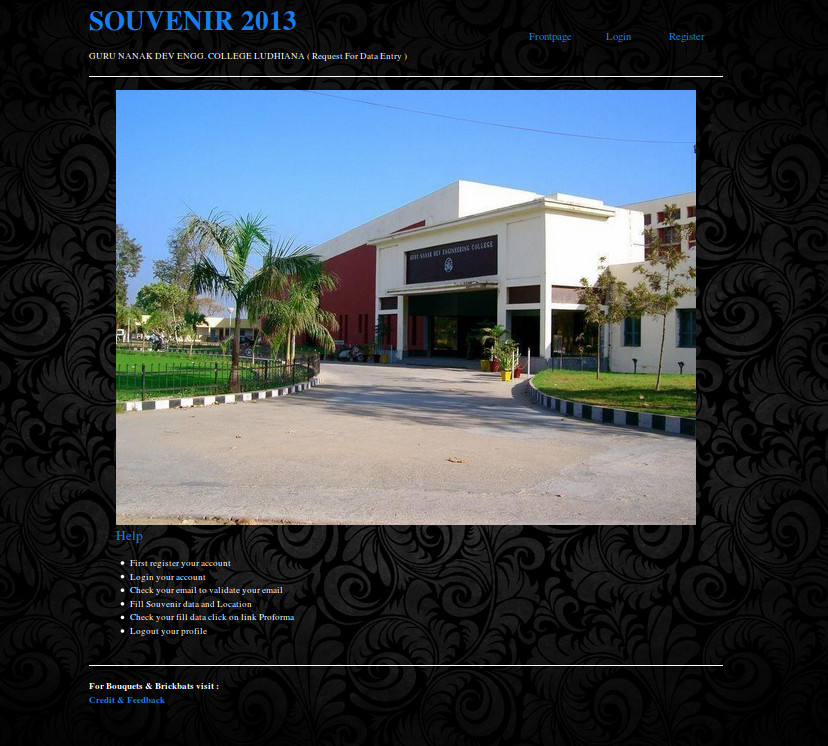
\includegraphics[width=0.6\textwidth]{images/fp.png}
\caption{Souvenir}
\end{figure}
Yaadein software woks in following different steps
\begin{itemize}
\item Fetching of data from the database.
\item Typesetting of data.
\item Including graphics.
\item Creating DVI file.
\item Creating post script file.
\item Creating pdf file.
\item Imposition of the pdf.
\item Color separation of the pdf(Optional)
\end{itemize}
Now let us discuss above points in detail
\subsubsection{Fetching of data from the database}
As for making SOUVENIR all the information required like student personal information, contact details,etc. were needed to be stored somewhere so phpMyAdmin was used
fo this purpose.\\
phpMyAdmin is a free software tool written in PHP intended to handle the\\
\image{0.5}{images/phpadmin.png}{phpMyAdmin logo}
administration of MySQL over the World Wide Web. phpMyAdmin supports a wide range of operations with MySQL. The most frequently used operations are supported by the user interface (managing databases, tables, fields, relations, indexes, users, permissions, etc), while you still have the ability to directly execute any SQL statement.\\
phpMyAdmin had already become one of the most popular PHP applications and MySQL administration tools, with a large community of users and contributors. In order to co-
ordinate the growing number of patches, a group of three developers registered The phpMyAdmin Project at SourceForge.net and took over the development in 2001.
Features.\\\\
\begin{itemize}
\item Web interface.
\item MySQL database management.
\item Import data from CSV and SQL.
\item Export data to various formats: CSV, SQL, XML, PDF (via the TCPDF library), ISO/IEC 26300 - OpenDocument Text and Spreadsheet, Word, Excel, \LaTeX{} and others.
\item Administering multiple servers.
\item Creating PDF graphics of the database layout.
\item Creating complex queries using Query-by-example (QBE).
\item Searching globally in a database or a subset of it.
\item Transforming stored data into any format using a set of predefined functions, like displaying BLOB-data as image or download-link.
\item Active query monitor (Processes).
\end{itemize}
Fetching data from the database and this is done through php programmming. PHP initially makes a connection with database before fetching teh data.
\begin{verbatim}
<?php
$conn = mysql_connect("localhost", $userName, $passWord);
mysql_select_db($DB);
?>
\end{verbatim}
\subsubsection{Typesetting of data}
Second step after fetching data was indeed to fit that at right place for which \LaTeX{} was used. \LaTeX{} is Type Setting editor. Lots of things were tried to make the look of the document better from tables to frame alast psframebox were used to set the data.
\begin{verbatim}
\psframebox*[par]{stuff}
\end{verbatim}
A simple frame (perhaps with rounded corners) is drawn using
\begin{verbatim}
\psframe
\end{verbatim}
The * option is of particular interest. It generates a solid frame whose color is fillcolor (rather than linecolor, as with the closed graphics objects). Recall that the default value of fillcolor is white, and so this has the effect of blotting out whatever is behind the
box. Small example\\
\image{0.4}{images/record.png}{Record of students}\\
\begin{verbatim}
\rput(1.2;35){\psframebox*{\small\$9.0M}}
\uput{2.2}[45](0,0){Oreos}
\rput(1.2;135){\psframebox*{\small\$16.7M}}
\uput{2.2}[135](0,0){Heath}
\rput(1.2;280){\psframebox*{\small\$23.1M}}
\uput{2.2}[280](0,0){M\\&M}
\endpspicture
\end{verbatim}
\subsubsection{Creating a DVI file}
The Device independent file format (DVI) is the output file format of the TeX typesetting program, designed by David R. Fuchs in 1979.[1] Unlike the TeX markup files used to generate them, DVI files are not intended to be human-readable; they consist of binary data describing the visual layout of a document in a manner not reliant on any
specific image format, display hardware or printer. DVI files are typically used as input to a second program (called a DVI driver) which translates DVI files to graphical data. For example, most TeX software packages include a program for previewing DVI files on a user’s computer display; this program is a driver. Drivers are also used to convert from DVI to popular page description languages (e.g. PostScript, PDF) and for printing.\\\\
DVI differs from PostScript and PDF in that it does not support any form of font embedding. (Both PostScript and PDF formats can either embed their fonts inside the
documents, or reference external ones.) For a DVI file to be printed or even properly previewed, the fonts it references must be already installed. Also, unlike PostScript, DVI is not a full, Turing-complete programming language, though it does use a limited sort of machine language.\\
Command :\$ latex file name
\subsubsection{Creating a postscript file}
PostScript (PS) is a dynamically typed concatenative programming language created by John Warnock and Charles Geschke in 1982. PostScript is best known for its use as a
page description language in the electronic and desktop publishing areas.\\\\
The concepts of the PostScript language were seeded in 1976 when John Warnock was working at Evans \& Sutherland, a computer graphics company. At that time John Warnock was developing an interpreter for a large three-dimensional graphics database of New York harbor. Warnock conceived the Design System language to process the graphics.\\
\image{0.5}{images/typesetting.png}{Type-setting using tables}\\

Command: \$ dvips file name -o

\subsubsection{Use In Printing}
Prior to the introduction of PostScript, printers were designed to print character output given the texttypically in ASCIIas input. There were a number of technologies for this task, but most shared the property that the glyphs were physically difficult to change, as they were stamped onto typewriter keys, bands of metal, or optical plates.\\\\
PostScript printing\\
PostScript went beyond the typical printer control language and was a complete programming language of its own. Many applications can transform a document into a PostScript
program whose execution will result in the original document. This program can be sent to an interpreter in a printer, which results in a printed document, or to one inside another application, which will display the document on-screen. Since the document-program is the same regardless of its destination, it is called device independent.\\

\image{0.4}{images/psbox.png}{Type-setting using psframebox}

\subsubsection{Creating a PDF file}
Portable Document Format (PDF) is an open standard for document exchange. This file format created by Adobe Systems in 1993 is used for representing documents in a manner independent of application software, hardware, and operating systems.Each PDF file encapsulates a complete description of a fixed-layout flat document, including the text, fonts, graphics, and other information needed to display it.\\\\
The PDF combines three technologies:\\
\begin{itemize}
\item A subset of the PostScript page description programming language, for generating the layout and graphics.
\item A font-embedding/replacement system to allow fonts to travel with the documents.
\item A structured storage system to bundle these elements and any associated content into a single file, with data compression where appropriate.
\end{itemize}
Command: \$ ps2pdf file name.ps\\
\image{0.4}{images/device.png}{Device Independent File}

\subsubsection{Imposition of the pdf}
Imposition is one of the fundamental steps in the prepress printing process. It consists in the arrangement of the printed product’s pages on the printer’s sheet, in order to obtain faster printing, simplify binding and reduce paper waste.\\
Correct imposition minimizes printing time by maximizing the number of pages per impression, reducing cost of press time and materials. To achieve this, the printed sheet must be filled as fully as possible.\\\\
Below code will convert and merge two pdf files on single page eg:
\image{0.2}{images/imp.png}{Imposition of pdf files}
\begin{verbatim}
\documentclass{article}
\pdfpagewidth 283mm
\pdfpageheight 460mm
\usepackage[pdftex]{color,graphicx,epsfig}
\usepackage[paperwidth=283mm,paperheight=460mm,left=0cm,top=0cm,bottom=0cm,right=0cm]{geometry}
\usepackage[final]{pdfpages}   %for including pdf files 
\begin{document}
\includepdf[pages=-, signature=8,landscape]{cover8.pdf}  %Cover8 folder contains all pdf files without imposition
\end{document}
\end{verbatim}
After merging two pdf pages on single page, next we have to do imposition of pages in such a way that after folding that pdf sheet front-inside,front-outside,back-inside and back-outside goes to their respective position.
\begin{verbatim}
\documentclass{article}
\pdfpagewidth 460mm
\pdfpageheight 566mm
\usepackage[pdftex]{color,graphicx,epsfig}
\usepackage[paperwidth=460mm,paperheight=566mm,left=0mm,top=0mm,bottom=0mm,right=0mm]{geometry}    
\usepackage[final]{pdfpages}
\begin{document}
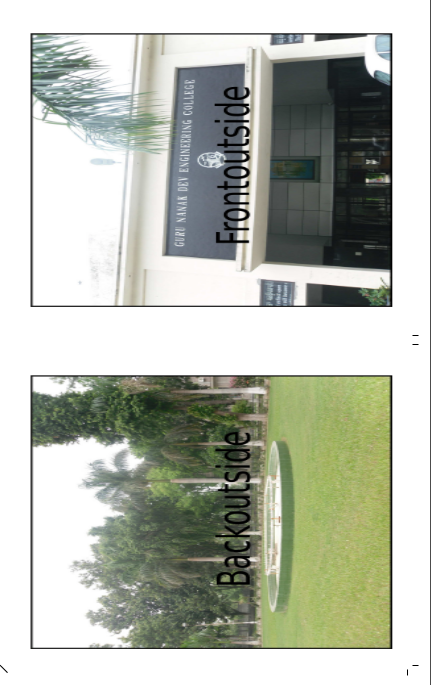
\includepdf[pages=-, signature=4,landscape]{imp.pdf}
\end{document}
\end{verbatim}
This will typeset the pages on their respective position eg:\\
\image{0.3}{images/imp2.png}{Final Imposition}
\newpage
\subsubsection{Color separation of the pdf}
Color printing or Colour printing is the reproduction of an image or text in color (as opposed to simpler black and white or monochrome printing). Any natural scene or color photograph can be optically and physiologically dissected into three primary colors, red, green and blue, roughly equal amounts of which give rise to the perception of white, and different proportions of which give rise to the visual sensations of all other colors. The additive combination of any two primary colors in roughly equal proportion gives rise to the perception of a secondary color. For example, red and green yields yellow, red and blue yields magenta (a purple hue), and green and blue yield cyan (a turquoise hue). Only yellow is counter-intuitive. Yellow, cyan and magenta are merely the "basic" secondary colors: unequal mixtures of the primaries give rise to perception of many other colors all of which may be considered "tertiary."
\subsubsection{RGB}
The RGB color model is an additive color model in which red, green, and blue light are added together in various ways to reproduce a broad array of colors. The name of the model comes from the initials of the three additive primary colors, red, green, and blue.\\\\
The main purpose of the RGB color model is for the sensing, representation, and display of images in electronic systems, such as televisions and computers, though it has also been used in conventional photography. Before the electronic age, the RGB color model already had a solid theory behind it, based in human perception of colors.\\
\image{0.3}{images/rgb.png}{RGB color}

\subsubsection{CMYK}
The CMYK color model (process color, four color) is a subtractive color model, used in color printing, and is also used to describe the printing process itself. CMYK refers to the four inks used in some color printing: cyan, magenta, yellow, and key (black). Though it varies by print house, press operator, press manufacturer, and press run, ink is typically applied in the order of the abbreviation.The "K" in CMYK stands for key because in four-color printing, cyan, magenta, and yellow printing plates are carefully keyed, or aligned, with the key of the black key plate.\\
The CMYK model works by partially or entirely masking colors on a lighter, usually white, background. The ink reduces the light that would otherwise be reflected. Such a model is called subtractive because inks "subtract" brightness from white.In additive color models such as RGB, white is the "additive" combination of all primary colored lights, while black is the absence of light. In the CMYK model, it is the opposite: white is the natural color of the paper or other background, while black results from a full combination of colored inks.
\image{0.3}{images/cmyk.png}{CMYK color}

\subsubsection{RGB to CMYK}
\image{0.7}{images/rgbcmyk.jpeg}{RGB and CMYK difference}
\hspace{-1.8em} A comparison of RGB and CMYK color spaces. The image demonstrates the difference between the RGB and CMYK color gamuts. The CMYK color gamut is much smaller than the RGB color gamut, thus the CMYK colors look muted. If you were to print the image on a CMYK device (an offset press or maybe even a ink jet printer) the two sides would likely look much more similar, since the combination of cyan, yellow, magenta and black cannot reproduce the range (gamut) of color that a computer monitor displays. This is a constant issue for those who work in print production. Clients produce bright and colorful images on their computers and are disappointed to see them look muted in print.\\\\
How to convert RGB to CMYK?\\\\
First we need imagemagick. Install it using following command:\\\\
\$ sudo apt-get install imagemagick\\\\
Following commands convert the rgb pdf file  to cmyk\\
1. Check whether the final.pdf is rgb or cmyk\\
\$ identify -verbose ‘final.pdf’\\\\
It displayes the many properties. Check colorspace: rgb /cmyk\\
\image{0.2}{images/r1.png}{RGB Check}\\
If it displayes cmyk, then its ok. Otherwise need to convert into cmyk\\\\
2. To convert rbg to cmyk use following command:\\\\
\$ gs -dSAFER -dBATCH -dNOPAUSE -dNOCACHE -sDEVICE=pdfwrite -sColorConversionStrategy=CMYK -dProcessColorModel=/DeviceCMYK -sOutputFile=output.pdf input.pdf\\
\begin{verbatim}
NOTE:- input.pdf = your_file_name.pdf
output.pdf = output_pdf_file.pdf
It displays the following output:
\end{verbatim}
\image{0.2}{images/r2.png}{RBG to CMYK page convertion}
Replace the input.pdf with your test pdf file\\
3. Now again check the properties of pdf file by following command:\\
\$ identify -verbose 'test.pdf'\\
It displays the following output:\\
\image{0.2}{images/r3.png}{CMYK converted pages}\\

\subsection{Evaluation and Maintenance}
Implementation is the process of having systems personnel check out and put new equipment into use, train users, install the new application and construct any files of data
needed to use it. This phase is less creative than system design. Depending on the size of the organization that will be involved in using the application and the risk involved
in its use, systems developers may choose to test the operation in only one area of the firm with only one or two persons. Sometimes, they will run both old and new system
in parallel way to compare the results. In still other situations, system developers stop using the old system one day and start using the new one the next.\\
Evaluation of the system is performed to identify its strengths and weaknesses. The actual evaluation can occur along any of the following dimensions:\\
\begin{itemize}
\item Operational Evaluation: Assessment of the manner in which the system functions, including case of use, response time, overall reliability and level of utilization.
\item Organizational Impact: Identification and measurement of benefits to the organization in such areas as financial concerns, operational efficiency and competitive impact.
\item User Manager Assessment: Evaluation of the attitudes of senior and user manager within the organization, as well as end-users.
\item Development Performance: Evaluation of the development process in accordance with such yardsticks as overall development time and effort, conformance to budgets.
\end{itemize}
\image{0.3}{images/device_indp.png}{Device Independent File Created}
and standards and other project management criteria.\\\\
Maintenance is necessary to eliminate errors in the working system during its working life and to tune the system to any variations in its working environment often small system deficiencies are found as a system is brought into operations and changes are made to remove them. System planners must always plan for resource availability to carry out these maintenance functions. The importance of maintenance is to continue to bring the new system to standards.\\
\image{0.3}{images/ps.png}{Post Script File Created}
\newpage
\subsection{RGB To CMYK Example :-}
\begin{figure}[h!]
\centering
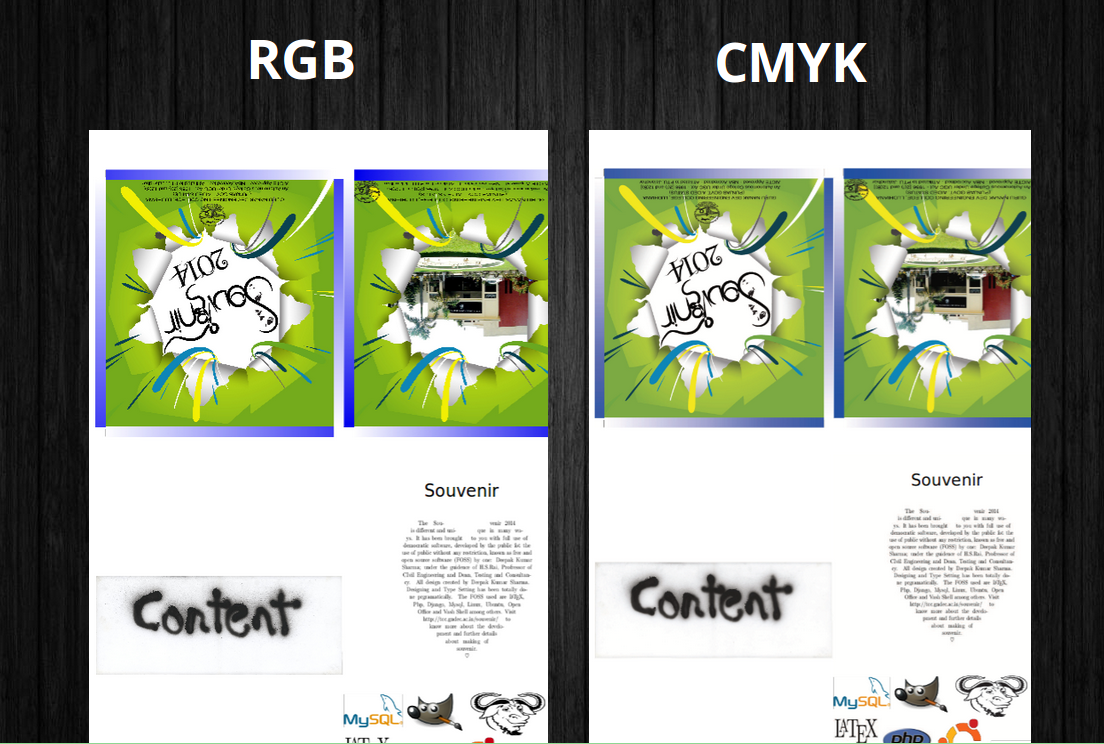
\includegraphics[width=0.8\textwidth]{images/rc.png}
\caption{RGB To CMYK}
\end{figure}

\newpage
\section{Results and Discussions}
\begin{itemize}
\item The results of the project work have been depicted in the Figure below. The results depict that almost ninety percent of the time is being saved when we use automation. This not only helps to increase efficiency but also enhances the work experience of the user.
\item The graphics used in the application are made using GIMP v2.6 which supports batch processing of images and thus acts as a great added advantage when several image files have to be processed simultaneously. This saves time and effort required to modify each file individually. Also by setting the properties of the various layers of the images during making the graphics for the souvenir, we can increase or decrease the quality of the images according to our requirements.
\item Use of very high quality graphics increases the running time of the application as such graphics have large file sizes and thus affect the processing time immensely especially during the making of the adobe postscript format file which is further converted to the pdf format after highly compressing the file. In case of the test data used by us, we used 20 MB graphics for covers(8 pages) and 40 MB files for backgrounds(78 pages) and thus ended up with a 2 GB postscript file which was further compressed to a 35 MB PDF file. In another instance, we used 2 MB graphics for both cover pages as well as separator pages. This gave us a 180 MB postscript file which was further compressed to a 3.1 MB pdf file. Thus, size of the graphics plays a major role in the processing time and disk space usage requirements.
\image{0.2}{images/All.png}{All Files Created}
\item postscript file which was further compressed to a 3.1 MB pdf file. Thus, size of the graphics plays a major role in the processing time and disk space usage requirements.
\item The application can also be made light weight by using small sized graphics which
will not only reduce running time but also save time on making them as not much effort will be needed to make them. Application of pictures of students can be done through a simple code snippet that might be included in the main script itself or might be added as a separate utility that has to be run by the user before the main script is run.
\item The time measurements and comparisons have been done in seconds and thus the accuracy of these might vary under different test conditions.
\image{0.3}{images/2.png}{Cover Page}
\end{itemize}
\newpage
\section{Conclusion and Future Scope}
\subsection{Conclusion}
Yaadein is an very efficient application which help in generating booklet for pass out student. It can be used 
by schools, colleges, universities, etc. It is
less time consuming and user friendly. It has been successfully used
in our college.
\subsection{Current status}
Yaadein is web based application. It will generate booklet passing through various stages:
\begin{itemize}
\item Web based user Interface for filling user-name, room, roll no, address, comments etc.
\item Data retrieved by using php connextivity with database.
\item Typesetting of pages usinf \LaTeX{}.
\item Imposition of pages using \LaTeX{}.
\item Color seperation i.e RGB to CMYK.
\end{itemize}
\subsection{Scope}
\begin{itemize}
\item The Yaadein project has already improved the Souvenir making experience to a huge extent by automating the making process, reducing the time tremendously from several weeks to a few minutes(may vary depending on the processor of the system in use) and cutting costs hugely.
\item By the use of complete open source technologies and cutting dependence on proprietary software such as the ever so expensive Adobe Photoshop, Microsoft Windows, Microsoft SQL, Microsoft office, etc. among others.
\item Although automated to a large extent, Yaadein is still in its initial development stages and there is still scope for a lot of development.
\item We plan to add a lot of other features some of which are automated imposition and colour separation for printing press requirements, automated design templates
for improving the aesthetic beauty of the souvenir, graphical interface for the non-terminal savvy users who will be able to make the souvenir without the use of the terminal.
\item We plan to provide hosting and remote access facilities for those users who do not have supporting hardware and software for running the application.
\end{itemize}

\newpage
\section{Coding}
\subsection{}
\subsection{PHP coding}
\begin{verbatim}
<?
include("db.php");
include("raiSED.php");

function correct_address($wrong_address) {
	$add1_arr = explode(",",$wrong_address);
		foreach($add1_arr as $addr) {
			$add_vpo = explode(" ",$addr);
			foreach($add_vpo as $add_vp) {
				if($add_vp=='V.P.O' or $add_vp=='vpo' or $add_vp=='VPO' or $add_vp=='Vpo' or $add_vp=='V.P.O.' or $add_vp=='V.P.O-' or $add_vp=='v.p.o.' or $add_vp=='v.p.o' or $add_vp=='v po') {
					$add_vpt = str_replace(".","",$add_vp);
					$add_vptt = strtoupper($add_vpt);
				}
				else {
					$add_vptt=$add_vp;
				}
				$add_VP[] = $add_vptt;
			}
			$add_VPO = implode(" ",$add_VP);
			unset($add_VP);
			$add1[] = ucwords($add_VPO);
		}
		$address1 = implode(",",$add1);
		unset($add1);
	return $address1;
}


$OneBranch ='information';
//echo"\section{{$OneBranch}}";
//echo"\\";
//echo"\section{ $OneBranch } \\\";
$PrintFlag = 0 ;                                                         // Print messages during development, if it is !=0

$PageWidth = 17.8; $PageHeight = 22.13;                                     //Page specifications

$CommentX = 0; $CommentY = -6; $CommentWidth = "8.5cm";               //Comment Specifications

$PerInfoWidth = "5.5cm";						    //Basic Info. Width

$GapX = "0.0"; $Gap2X = "1.2" ;
$CoorX ="-1.2" ;

$PhotoX = 1; $PhotoY = 0; $PhotoWidth = "2.2cm";$PhotoHeight="3.5cm";   //Photo specifications

$itemInSequence = 8 ;                                                  // Name, FN, MN, address, Email etc

$pagecounter=48;
$tox= 0; $toy = 0; 

$OffSetX = 0; $StartX = 0 ; $ScaleX = 1;                                 //X-coord of the page
$OffSetY = 0; $StartY = $PageHeight; $ScaleY = 1;                      //Y-coord of the page

$Columns = 2; $Rows = 5; $RecordPerPage = $Columns * $Rows;             //No. of rows,columns and records on one page

$RecordFrom = 0;

$BoxX = $PageWidth / $Columns; $BoxY = $PageHeight / $Rows;		// X and Y coord. of a box of single record


for ($i = 0 ; $i < 20 ; $i++)
{
 $flagSED[$i] = 0;
}

$flagSED[5] = 1;               // Perfoem SED on address1
$flagSED[6] = 1;              // Perfoem SED on email
$flagSED[7] = 1;             // Perfoem SED on contact
$flagSED[8] = 1;            // Perfoem SED on comments
$flagSED[9] = 1;           // Perfoem SED on Photo



$PhotoPath = "/home/dk/Documents/so/souvenir/files/";

include("querydav.php");
//$sqlquery .= "limit 10 ";
//$Onebranch=$row[11];
//echo"\chapter*{{$OneBranch}}";
//echo"\pagebreak";

// echo $sqlquery;

$result = mysql_query($sqlquery);
$rows = mysql_num_rows($result);
$cols = mysql_num_fields($result);

$PagePerBranch = ceil( $rows / $RecordPerPage);




for ($page = 0; $page < $PagePerBranch; $page++)
{

// $RecordPerPage = 2;

$sqlQP2 = " order by class_roll_no limit $RecordFrom , $RecordPerPage ";  
$sqlQP1 = $sqltmp . $sqlQP2 ;

$result = mysql_query( $sqlQP1 );

$rows = mysql_num_rows($result);  
$cols=mysql_num_fields($result);  
if ( $PrintFlag !=0 ) echo $sqlQP1;
if ( $PrintFlag !=0 ) {echo "\n Row $rows \n $cols \n Page $page \n"; echo "";}

echo "\\begin{pspicture}($PageWidth,$PageHeight)";  
//echo "\includegraphics[width=\\textwidth,height=0.9cm]{sgeacheehead.eps}";
echo "\\rput[c|](8.9,22.7){{\includegraphics[width=22.2cm]{headfoot/sgeachithead.eps}}}";
echo "\\\\";


if($pagecounter%2==0)
{

echo "\\psline{-}(-2.8,-1.73)(-2.2,-1.73)";
echo "\\\\";
echo "\\psline{-}(-1.5,-2.33)(-1.5,-2.93)";
echo "\\\\";
}
else
{
echo "\\psline{-}(20,-1.73)(20.6,-1.73)";
echo "\\\\";
echo "\\psline{-}(19.4,-2.33)(19.4,-2.93)";
echo "\\\\";


}


$i = 0;
while ($i<$Rows)
{
$j = 0;
while ($j<$Columns)
{

if ( $PrintFlag !=0 ) echo "row: $i col : $j";

$BoxI1 = ($StartX +$j * $BoxX + $OffSetX)*$ScaleX ;
$BoxJ1 = ($StartY - $i * $BoxY + $OffSetY)*$ScaleY ;
$BoxI2 = ($StartX +($j+1) * $BoxX + $OffSetX)*$ScaleX ;
$BoxJ2 = ($StartY - ($i+1) * $BoxY + $OffSetY)*$ScaleY ;
$ii=$i+1; $jj=$j+1; 
//echo "\\rput($BoxI1,$BoxJ1){(($ii) X($jj))}";
echo"\n";
// echo"\psframe[fillcolor=lightgray]($BoxI1,$BoxJ1)($BoxI2,$BoxJ2)"; echo "\n";
$j++;
}
$i++;
}

echo "\n";
$i = 0; $j=0;
while (
$row = mysql_fetch_row($result)
//$row = mysql_fetch_assoc($result)
)
{


//$SEDi = 0;
//while ($row[$SEDi]) // for each field
for ($SEDi = 0; $SEDi < $cols; $SEDi++)
{
    $rowRai[$SEDi] = $row[$SEDi];
 if ($flagSED[$SEDi] != 0)
 {
//  $SEDj = 0;
//echo " $row[$SEDi] \n";
//  while ($OrgText[$SEDj])
  for ($SEDj=0; $SEDj < 14 ; $SEDj++)
  { 


    if ( $PrintFlag !=0 )  echo " SEDj $SEDj | inside sed \n";
   $rowRai[$SEDi] = str_replace($OrgText[$SEDj] , $ReplacedText[$SEDj] , $rowRai[$SEDi]);
//   $SEDj++;
  }
if ( $PrintFlag !=0 )   echo " $rowRai[$SEDi] outside sed \n"; 
//  $SEDi++ ;

}
}
    
// ================================================================= Basic personal information =============

echo "\\\\";
if ( $PrintFlag !=0 ) echo "row: $i col : $j";
 
$BoxI1 = ($StartX +$j * $BoxX + $GapX + $OffSetX)*$ScaleX ;
$BoxJ1 = ($StartY - $i * $BoxY + $OffSetY)*$ScaleY ;
$BoxI2 = ($StartX +($j+1) * $BoxX + $OffSetX)*$ScaleX ;
$BoxJ2 = ($StartY - ($i+1) * $BoxY + $OffSetY)*$ScaleY ;
$ii=$i+1; $jj=$j+1; 

$item = 0;

$Bx[$item] = $BoxI1+$tox + $PhotoWidth + ( ( ($PageWidth / $Columns) - $PhotoWidth) / 2.) + $Gap2X;
$By[$item] = $BoxJ1+$item * $toy;
$tempCorr = $Bx[$item] + $CoorX ;
//echo "\\rput[t|]($tempCorr ,$By[$item])";
//echo "{\psframebox{\parbox[l]{{$PerInfoWidth}}{\\raggedright ";
for ($item = 0; $item < $itemInSequence; $item++)
{
//echo $rowRai[$item]; 
echo " ";
//echo " \\\\ \n";
}
//echo "}}}\n";

$Ix=$BoxI1+$PhotoWidth+2.5;

$Iy=$BoxJ1+$toy;

//echo "\\rput[t|]($Ix ,$Iy)";
//echo "{\psframebox*{\parbox[l]{{$PerInfoWidth}}{\\raggedright ";
$linegap=0.3;
$Bxx = $BoxI1+$PhotoWidth+3.; $Byy = $BoxJ1+$toy; //NAME
$Gy=$Byy-2*$linegap; 		//Gender
$Fy=$Gy-2*$linegap;  		//Fname       
$My=$Fy-2*$linegap;  		//Mname
$Rx=$Bx; $Ry=$Fy-0.8;           //ROLL NO.
$ADy=$Ry-0.8;  		        //Address
$Dy=$ADy-0.8;  		        //DOB
$Ey=$Dy-0.6;  		        //Email
$CNy=$Ey-0.6;   	        //Cntctno.

$row[2]=ucwords(strtolower($row[2]));
$row[2] = str_replace(" ","~",$row[2]);

$row[1]=ucwords(strtolower($row[1]));
$row[1] = str_replace(" ","~",$row[1]);

echo "\\rput[t|]($Bxx,$Byy){";
echo "{\psframebox[linecolor=white,linestyle=dotted,dotsep=100pt,linewidth=0pt]{\parbox[l]{{$PerInfoWidth}}{\\raggedright ";
//echo "Name: ";
echo ucwords(strtolower($row[0])); echo " ("; echo $row[3] ; echo  ")"; 
if ($row[10]=="M")
echo " S/o ";
else
echo " D/o ";echo $row[2]  ; echo  " and "; echo $row[1] ;
echo "\\\\DoB: " ; echo date(' jS  F Y ', strtotime($row[4])); echo " ";
echo"\mbox{";echo $rowRai[6],"}"; echo " "; echo"\\\\Ph. "; echo $rowRai[7]; echo "\\\\";

$address_correct = correct_address($rowRai[5]);
echo $address_correct;
//echo $rowRai[11];
echo "}";
echo "}}}\n";


// Coordinates of Photo and Comment ==================================================================

$Cx = ( $Bx[0]+$CommentX + $OffSetX ) * $ScaleX ;
$Cy = ( $By[0]+$CommentY + $OffSetY ) * $ScaleY ;
$Cnewx=$BoxI1+$PhotoWidth+$PhotoWidth/2.+1.;
$Cnewy=$BoxJ1-3.45;
$Px = ( $Bx[0]+$PhotoX + $OffSetX ) * $ScaleX ;
$Py = ( $By[0]+$PhotoY + $OffSetY ) * $ScaleY ;
//$P1x=$Px+1.4;
//$P1y=$Py+0.1;
$Py1=$BoxJ1-3.5;
$Px1=$BoxI1+2.55;
// Photo here

$PhotoName = $rowRai[3];
$PhotoName = $row[3];
$PhotoNE = explode(".", $PhotoName);
$PhotoEPS = "files/S2013" .$PhotoNE[0] . ".eps" ;
// ===================================================== Photo ===============
//$PhotoURL = $PhotoPath . $PhotoEPS ;
$PhotoURL = $PhotoEPS ;
//echo"\psframe*($Px1,$Py1)($BoxI1,$BoxJ1)";
 //echo "\n";

$Pnew1=$BoxI1+$PhotoWidth/2.;
$Pnew2=$BoxJ1-0.02;
echo "\\rput[t|]($Pnew1,$Pnew2)";
echo "{\psframebox[framesep=0pt,boxsep=false,linecolor=white]{\parbox[c]{{$PhotoWidth}}{\\raggedright ";
echo "{\includegraphics[width=$PhotoWidth]{{$PhotoURL}}";

//echo "{\includegraphics[width=$PhotoWidth]{{$PhotoURL}}";
//echo "{\includegraphics[width=$PhotoWidth]{{files/kinda.eps}}";
echo "}}}";
echo "}\n";

// ===================================================== Comment =================
echo "\\rput[t|]($Cnewx,$Cnewy)";
//echo "{\psframebox[framesep=1pt,boxsep=false,linewidth=0pt,linestyle=dotted,linecolor=white]{\parbox[t]{{$CommentWidth}}{ ";
echo "{\psframebox[framesep=1pt,boxsep=false,linecolor=white,linestyle=dotted,dotsep=100pt,linewidth=0pt]{\parbox[t]{{$CommentWidth}}{";
echo $rowRai[8]; 
echo "}}}\n";
$j++;
if ($j >= $Columns) { $j = 0;  $i++; }
}
echo "\\rput[c|](8.9,-0.63){{\includegraphics[width=22.2cm]{headfoot/footer.eps}}}";
//echo $pagecounter;

echo "\\end{pspicture}";
//$pagecounter =$pagecounter++;
if ( ($page + 1 ) != $PagePerBranch) {echo "\n \pagebreak  \n";}

$RecordFrom += $RecordPerPage;
$pagecounter =$pagecounter + 1;
}

mysql_close();

?>
\end{verbatim}

\subsection{Main \LaTeX{} Code}
\begin{verbatim}
\documentclass[8pt,twoside]{extarticle}
\pdfpagewidth 230mm
\pdfpageheight 283mm

\usepackage{graphicx} 
\usepackage{pstricks}
\usepackage{color}
\selectcolormodel{cmyk}
\usepackage[paperwidth=230mm, paperheight=283mm, left=16.1mm, top=26.85mm, bottom=34.85mm, right=36.1mm]{geometry}
\usepackage{lastpage}
\usepackage{fancyhdr}
\usepackage{wallpaper}
\usepackage{shapepar}
\usepackage{layouts}
\usepackage{verbatim}
\usepackage{eso-pic}
\usepackage{xcolor}
\usepackage{blindtext}
\definecolor{maroon}{RGB}{185,0,0}
\setcounter{page}{15}

\begin{document}

\pagecolor{white}
\parindent=0pt

\include{filecivil}
\include{filecomputer}
\include{fileelectrical}
\include{fileelectronics}
\include{fileit}
\include{filemechanical}
\include{fileproduction}
\include{filemba}

\end{document}
\end{verbatim}
\newpage
\section{Bibliography}
\begin{thebibliography}{9}
\bibitem{} R.L. Graham, D.E. Knuth, and O. Patashnik, Concrete mathematics, Addison-Wesley, Reading, MA, 1989.
\bibitem{} Donald E. Knuth, The TeXbook, AddisonWesley, Boston, 1986, p. 1.
\bibitem{} Leslie Lamport (April 23, 2007). “The Writings of Leslie Lamport: LaTeX: A Docu-
ment Preparation System”.
\bibitem{} Welcome to the TeX Users Group web site
\bibitem{} Comprehensive TeX Archive Network (CTAN)
\end{thebibliography}

\begin{screen}
\newpage
\section{Links}
% http://202.164.53.116/~bhavneet/messages
\newline
%http://202.164.53.116/~bhavneet/Web
\newpage
\begin{center}

\section*{Thank you}
\end{center}



\end{screen}

\end{document}
